\subsection{Multi-core Experimental Results}
\label{sec:empirical}

\begin{figure}[h]
\centering
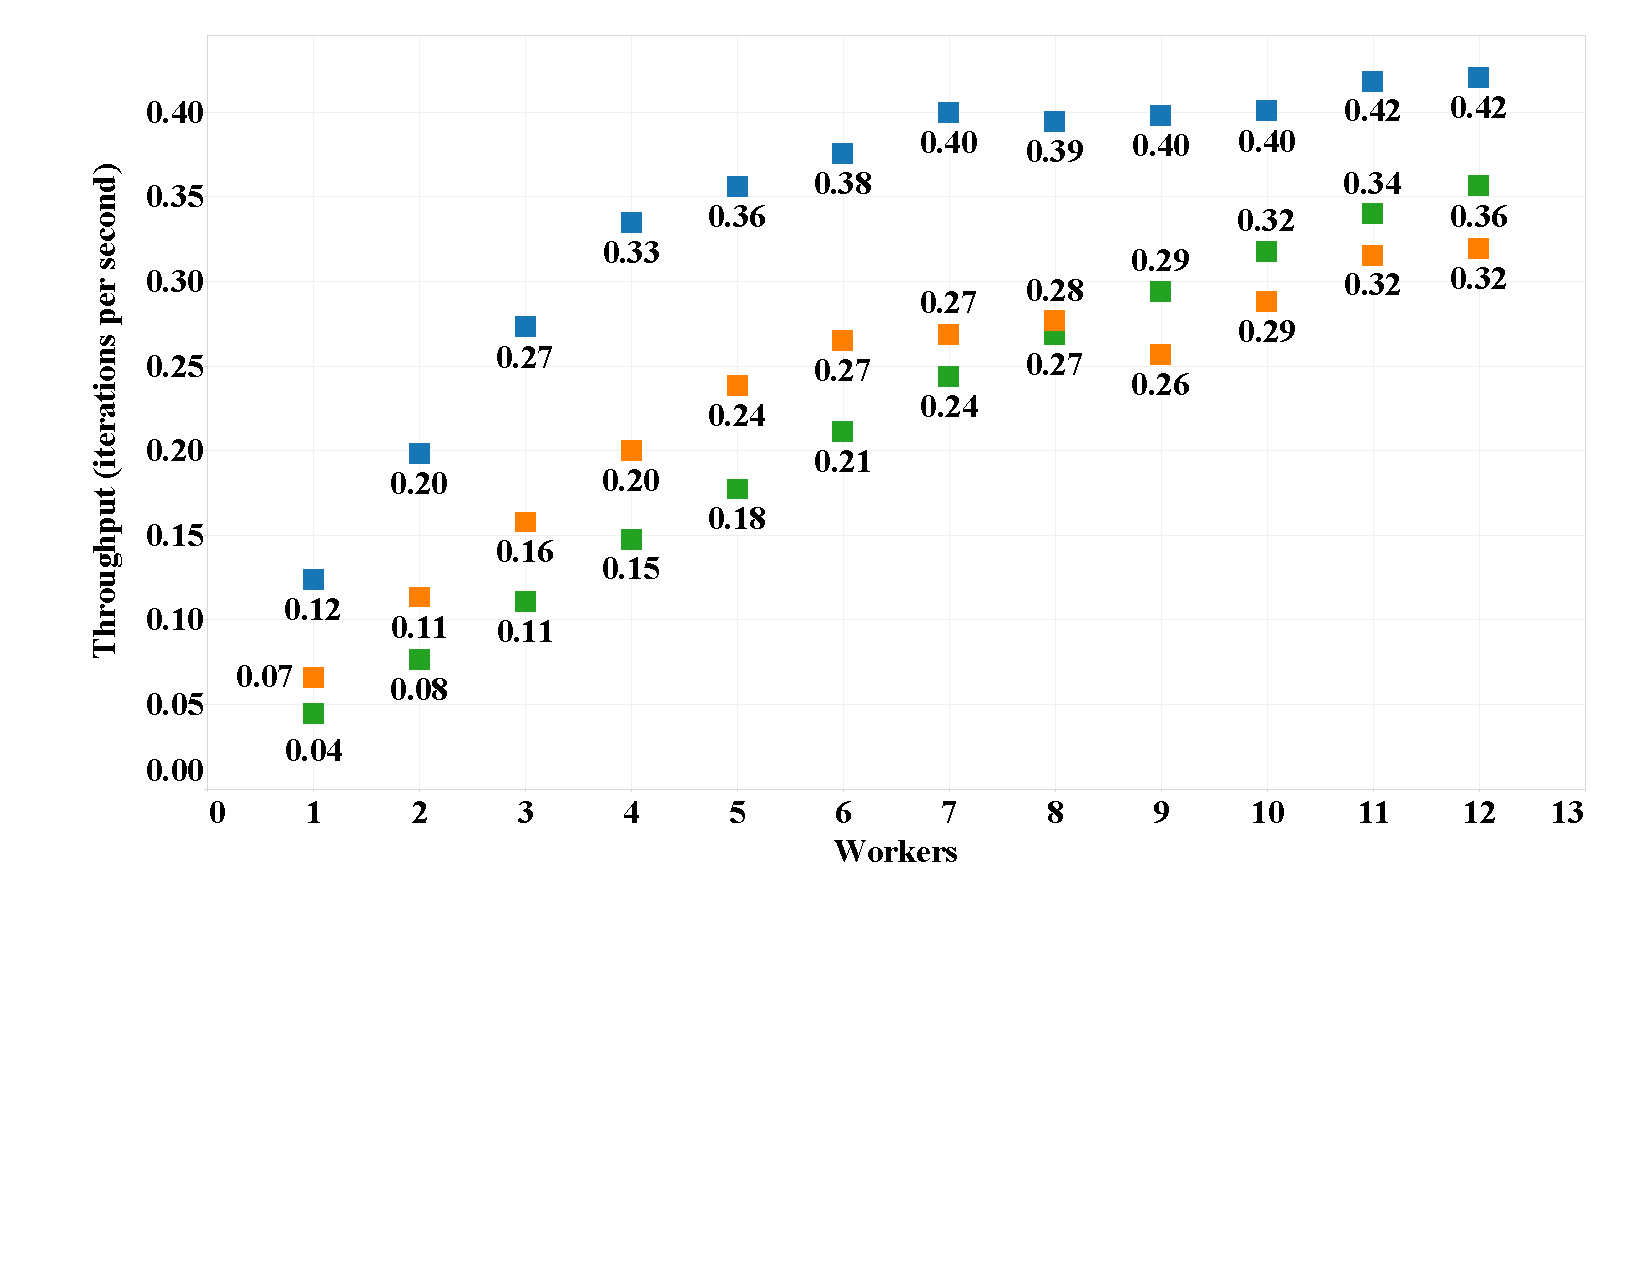
\includegraphics[width=5in,clip,trim=1cm 6cm 0 0]{figures/scalability_original.pdf}
\caption{Throughput vs. number of workers on the test graph 
with 50M vertices described in \secref{empirical}
for three scheduling algorithms: \proc{BSP} (i.e. blue), \proc{Laika} 
(i.e. orange) with $b=16$ 
(i.e. 65,536 vertices per chunk), and \proc{JonesPlassmann} (i.e. green).
}
\label{fig:scalability_original}
\end{figure}

\begin{figure}[h]
\centering
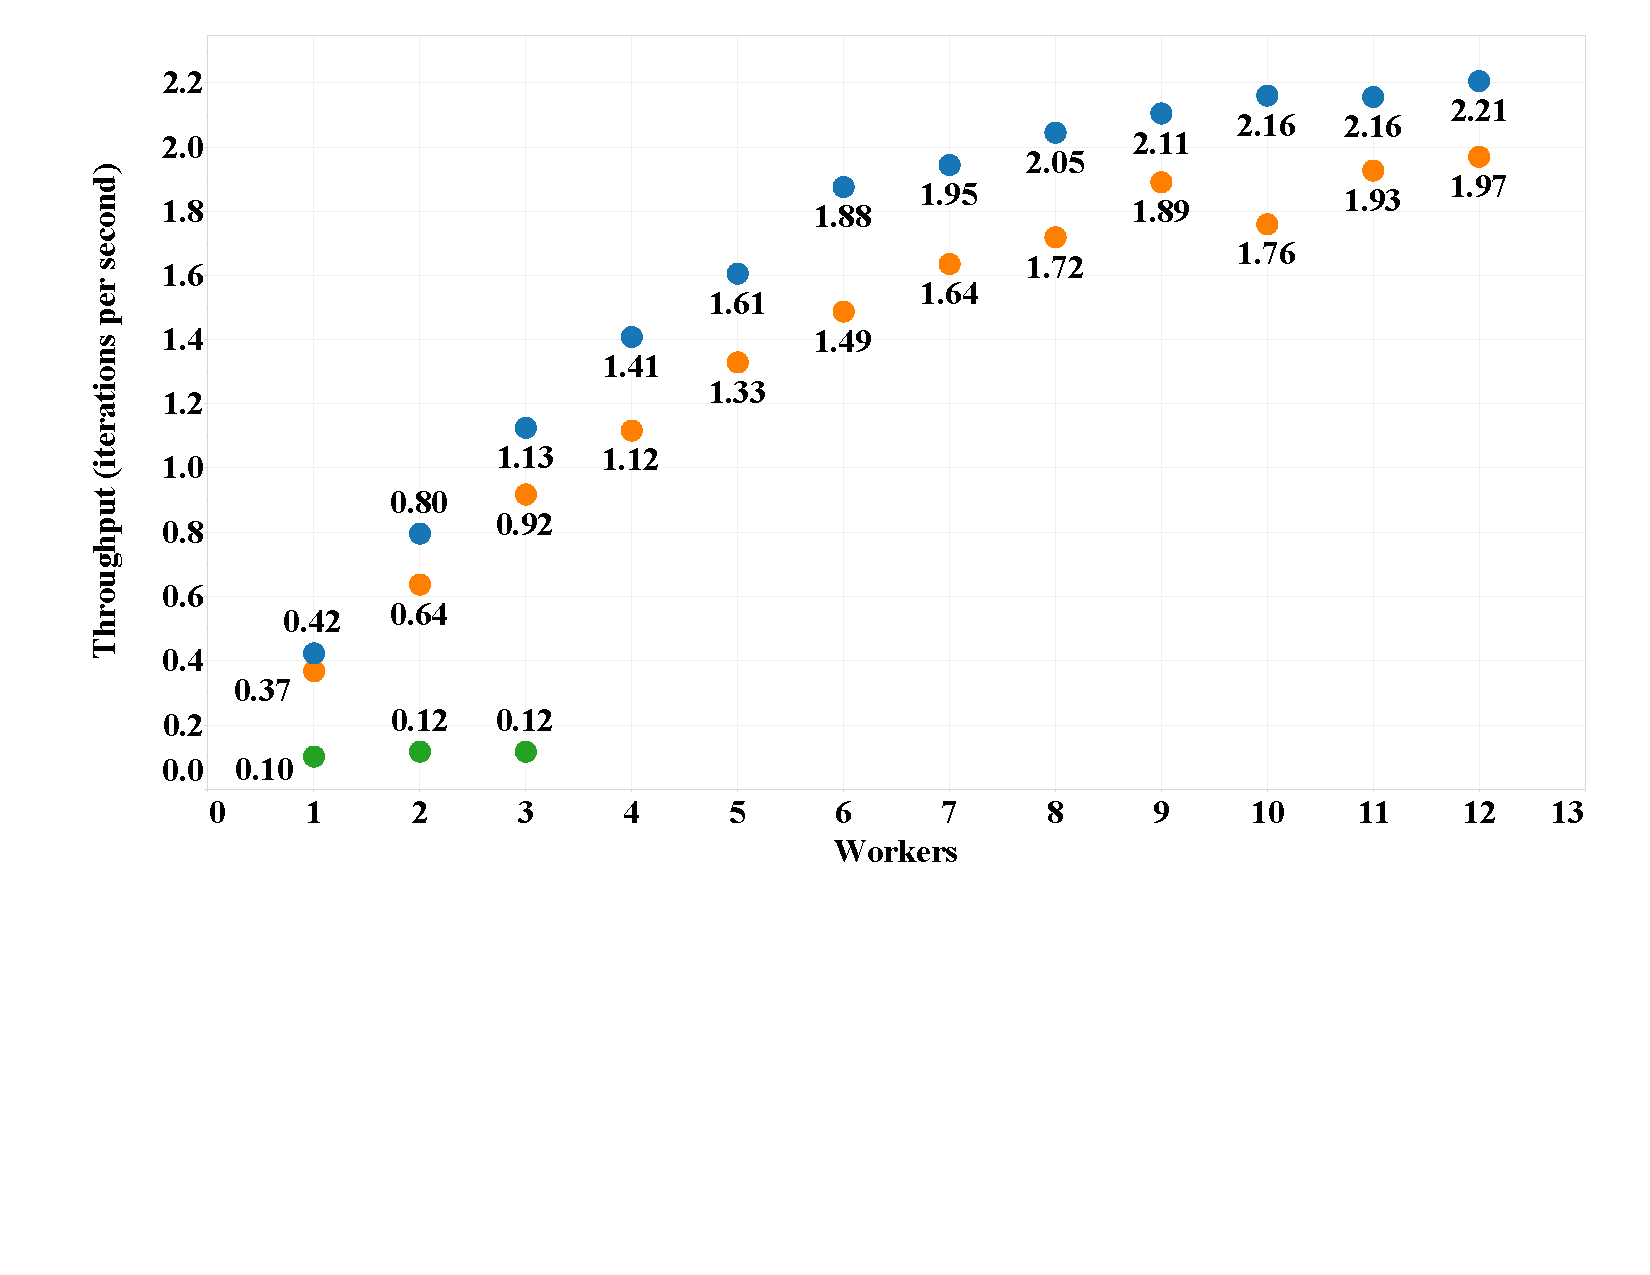
\includegraphics[width=5in,clip,trim=1cm 6cm 0 0]{figures/scalability_reordered.pdf}
\caption{Throughput vs. number of workers on the test graph 
with 50M vertices described in \secref{empirical} reordered
according to the Hilbert priority function
for three scheduling algorithms: \proc{BSP} (i.e. blue squares), \proc{Laika} (i.e. orange squares), and \proc{JonesPlassmann} (i.e. green squares).
}
\label{fig:scalability_reordered}
\end{figure}


We performed several experiments to characterize the scalability
of the \proc{BSP}, \proc{Laika}, and \proc{JonesPlassmann} scheduling
algorithms, the results of which are given in this section.  
We generated a random graph with 50M vertices uniformly
distributed on the unit cube with an
average degree of 16.4.  Edges are formed by joining any two vertices 
within a distance $r=\sqrt[\leftroot{-1}\uproot{1}3]{3\Delta/(4\pi n)}$, 
where $\Delta$ is the average degree and $n$ is the number of vertices.
\footnote{The value of $r$ follows from the fact that the expected 
number of neighbors $\Delta$ with $n$ vertices in the unit cube
is approximately $4\pi r^3 n/ 3$, the volume of a sphere of radius
$r$ times the number of vertices.}  This graph is used throughout
this section as a proxy for the type of locally-connected graphs
that we are likely to see from Simit.  In future work, we will
attempt to make synthetic generators of locally-connected 3D graphs
which have less regular shape and density.


\figref{scalability_original} shows throughput as a function of the number
of workers for the randomly ordered graph for the three scheduling
algorithms: \proc{BSP} (i.e. blue), \proc{Laika} (i.e. orange), and
\proc{JonesPlassmann} (i.e. green).  We can see that absent reordering
with good caching behavior \proc{Laika} is approximately equal to
\proc{JonesPlassmann} and scales worse.  This is not surprising, as 
\proc{Laika} is designed under the assumption that most of the edges
in the graph occur between pairs of vertices within the same $2^b$-vertex 
chunk.  

\figref{scalability_reordered} demonstrates the caching advantage realized
by reordering the vertices according to the Hilbert priority function
with $k=8$ (i.e. the unit cube is broken up into $2^k$ x $2^k$ x $2^k$ blocks).
We see that \proc{Laika} scales well and is within 10\% of the relative
ideal performance of \proc{BSP}.  Note that in order for \proc{BSP} to
be deterministic, the calculation must use double buffering of vertex state 
which would slow it down due to the extra memory usage, whereas the \proc{BSP} 
timings in \figref{scalability_reordered} do not use double buffering and
are thus not deterministic, but nonetheless serve as an approximate 
upper bound on performance of deterministic scheduling algorithms.  Notice
that \proc{JonesPlassmann} is missing data for greater than 3 workers.
In those cases, the experiments failed to complete due to an overflow of
stack space.  The recursive nature of \proc{JonesPlassmann} can lead to
problems of this sort when there are long dependency chains in the 
dag, which there are with reordering using the Hilbert priority function. 

\subsection{Effects of $k^\textrm{th}$-order Hilbert Reordering}
\label{sec:hilbert_bits}

\begin{figure}[h]
\centering
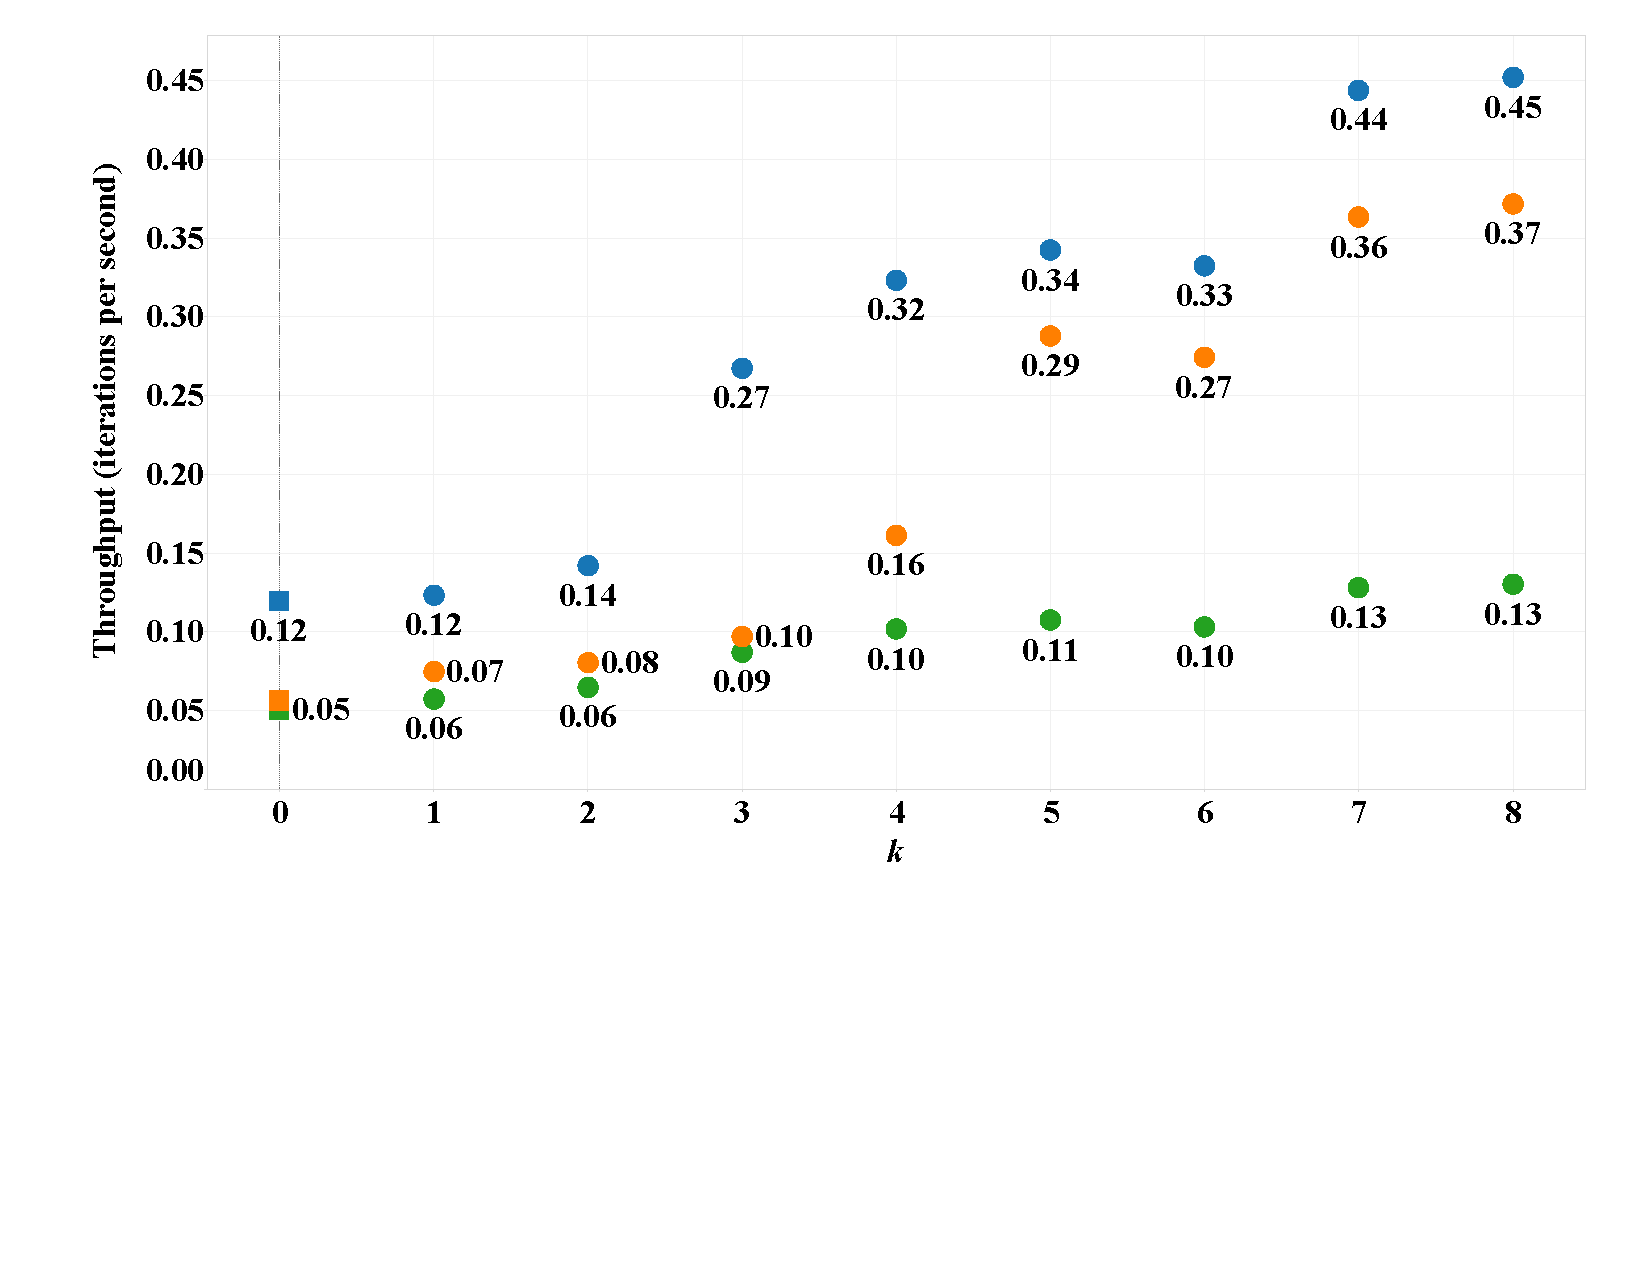
\includegraphics[width=5in,clip,trim=1cm 6cm 0 0]{figures/scalability_hilbert_bits_serial.pdf}
\caption{Throughput vs. $k$ on the 
test graph with 50M vertices described in \secref{empirical}
for three single-threaded scheduling algorithms: \proc{BSP} (i.e. blue), 
\proc{Laika} (i.e. orange), and \proc{JonesPlassmann} (i.e. green).
The value $k$ is an input parameter to the Hilbert 
priority function, which discretizes the unit cube into
a $2^k$ x $2^k$ x $2^k$ lattice where vertices lying within
the same lattice block are ordered randomly.  The
special case of $k=0$ (i.e. squares) indicates that the input 
graph consists of randomly ordered vertices.
}
\label{fig:scalability_hilbert_bits_serial}
\end{figure}

\begin{figure}[h]
\centering
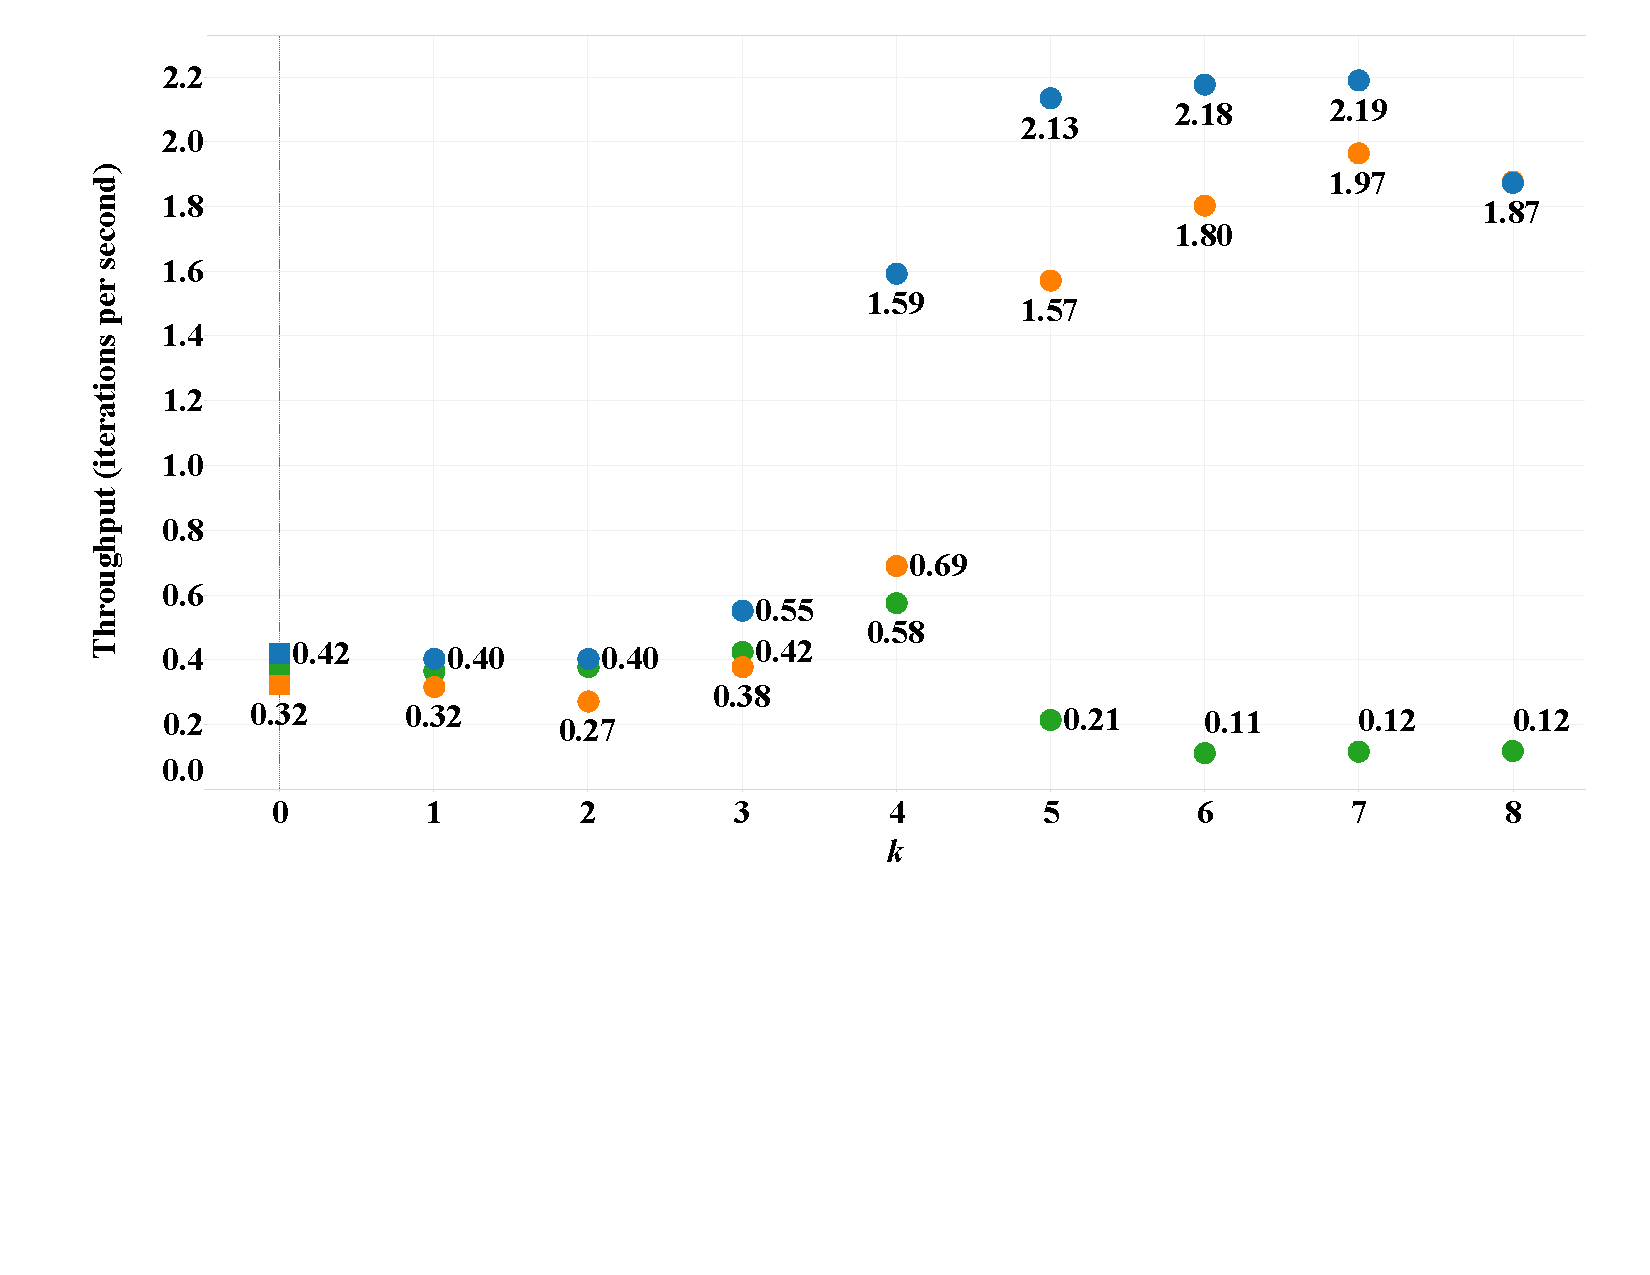
\includegraphics[width=5in,clip,trim=1cm 6cm 0 0]{figures/scalability_hilbert_bits_parallel.pdf}
\caption{Same as \figref{scalability_hilbert_bits_serial} except that
the scheduling algorithms are executed with 12 workers.}
\label{fig:scalability_hilbert_bits_parallel}
\end{figure}


In \figreftwo{scalability_hilbert_bits_serial}{scalability_hilbert_bits_parallel}
we see throughput as a function of $k$ for serial and parallel
executions, respectively.  As $k$ increases the granularity of the
Hilbert curve shrinks, which increases the caching advantage at
the expense of creating longer dependency chains.  Each vertex has
approximately 184 bytes of data associated with it (56 bytes in the
vertex array itself and 128 bytes in the edge array).  In 
\figref{scalability_hilbert_bits_serial} we see a big jump in
throughput between $k=4$ and $k=5$.  At $k=4$, there are $4096$
total blocks traced out by the Hilbert curve, each of which has
an average of ~2.2MB of state (i.e. 184 bytes times 50M vertices divided
by 4096 blocks).  However, throughput jumps at the point 
$k=5$ where the amount of state per block drops
by a multiple of 8 or roughly the size of the L2 cache.  We also
notice that due to its depth-first nature of the recursive formulation,
\proc{JonesPlassmann} fails to take advantage of the increased
cache locality offered by increasing the value of $k$.  In fact,
in \figref{scalability_hilbert_bits_parallel} we see that performance
actually decreases with increasing $k$ for \proc{JonesPlassmann},
likely due to the fact that longer dependency chains reduce the
parallelism in the computation.




